\documentclass{article}
\usepackage{graphicx}
\usepackage{amsthm}
\usepackage[english]{babel}
\begin{document}
\title{Rongpeng Li's part}
\section{Hadamard Product}
the Hadamard product (also known as the Schur product or the entrywise product is a binary operation that takes two matrices of the same dimensions, and produces another matrix where each element $ij$ is the product of elements $ij$ of the original two matrices.It is attributed to, and named after, either French mathematician Jacques Hadamard, or German mathematician Issai Schur.
The Hadamard product is commutative, associative and distributive over addition. That is
\begin{eqnarray}
        % \nonumber to remove numbering (before each equation)
          A*B &=& B*A \\
          A*(B*C) &=& (A*B)*C \\
          A*(B+C) &=& A*B+A*C
        \end{eqnarray}
The identity matrix under Hadamard multiplication of two m-by-n matrices is m-by-n matrix where all elements are equal to 1, which is different from simple identity matrix $I$\\
A matrix has an inverse under Hadamard multiplication if and only if none of the elements are equal to zero.\\
In programming language like MATLAB, Hadamard product is done by using $.*$ where $*$ stands for the normal multiplication.

\section{Properties of Hadamard Product}
For square $A$ and $B$, the row-sums of their Hadamard product are the diagonal elements of $AB^{T}$
\begin{equation}
\sum_{j}(A*B)_{i,j} = (AB^{T})_{i,j}
\end{equation}
\\
The Hadamard product is a principal submatrix of the Kronecker product.\\
A principal submatrix is a square submatrix where the distinguished rows and columns are the same.

\section{Schur Product Theorem}
\begin{theorem}
The Hadamard product of two positive-semidefinite matrices is positive-semidefinite. This is known as the Schur product theorem.
\end{theorem}
\begin{proof}
Proof is done using eigendecomposition.\\
Let $M = \sum u_{i}m_{i}m_{i}^{T} $ and $N = \sum v_{i}n_{i}n_{i}^{T}$. Then $M*N = \sum_{i,j} u_{i}v_{j}(m_{i}m_{i}^{T})*(n_{j}n_{j}^{T}) = \sum_{i,j} u_{i}v_{j}(m_{i}*n_{j})(m_{i}*n_{j})^{T}$.
Each $(m_{i}*n_{j})(m_{i}*n_{j})^{T}$ is positive and $u_{i}v_{j} >0$, thus the sum giving $M*N$ is also positive.
\end{proof}

\section{Product Rule for Hadamard Product}

\begin{theorem}
Suppose $Y$ and $X$ are $m-n$ matrices and each of whose elements is a differentiable function of all elements of a $p-n$ matrix Z. Then
\begin{equation}
\frac{\partial{(Y*X)}}{\partial{Z}} = \frac{\partial{Y}}{\partial{Z}}(D_{\hat{x}}) + \frac{\partial{X}}{\partial{Z}}(D_{\hat{y}}).
\end{equation}
\end{theorem}

\begin{proof}
\begin{equation}
\frac{\partial{Y}}{\partial{Z}}(D_{\hat{x}}) + \frac{\partial{X}}{\partial{Z}}(D_{\hat{y}}) = [\sum_{ij }(\frac{\partial{y_{ij}}}{\partial{z_{st}}}x_{ij})+\sum_{jk}(y_{jk}\frac{\partial{x_{jk}}}{\partial{z_{st}}})]
\end{equation}
By the definition of $D_{x}$,
\begin{equation}
RHS=\frac{\partial{(Y*X)}}{\partial{Z}}.
\end{equation}
\end{proof}


\section{Physical Meaning of Hadamard Product}
A very intuitive way to understand Hadamard product is to view it as a amplification of image processing.
Here is a demonstration of Hadamard product that reduces the brightness of a picture. The matrix of original picture Hadamard-multiplies another matrix of exponential decay from the center.

\begin{table}
  \centering
  \begin{tabular}{ l l l}

    % after \\: \hline or \cline{col1-col2} \cline{col3-col4} ...
    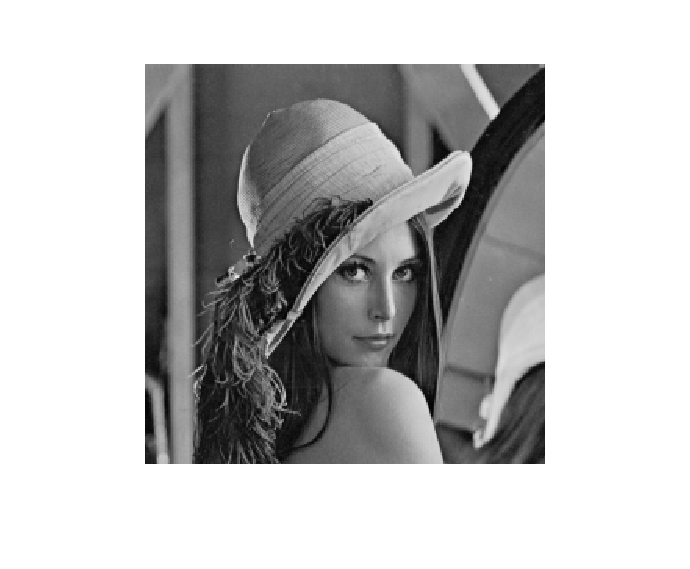
\includegraphics[width=4cm]{Original.eps} & \includegraphics[width=4cm]{H.eps} & 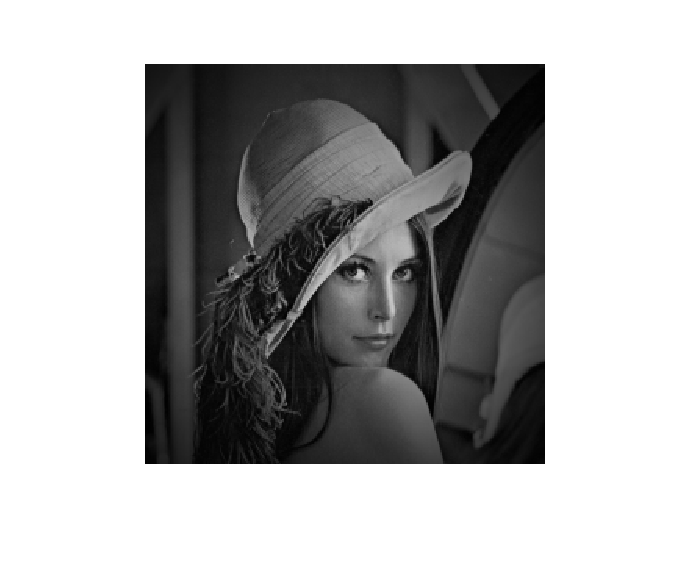
\includegraphics[width=4cm]{New.eps} \\

  \end{tabular}
  %\caption{}\label{}
\end{table}

\section{Hadamard Matrix}
The Hadamard matrix $H$ is a square with elements 1 or -1. It has several interesting properties.It is first studied by the same French mathematician.
\begin{equation}
HH^{T} = nI_{n}
\end{equation}
A Hadamard matrix has maximal determinant among matrices with entries of absolute value less than or equal to 1. If $M$ is a complex matrix of order n, whose entries are bounded by $M_{ij}\leq 1$, then $|det(M)| \leq n^{n/2}$.\\
The Hadamard matrix can be constructed by Sylvester's construction.
\section{Sylvester's construction}
If $H$ is a Hadamard matrix, then the matrix below is also a Hadamard matrix.
$
\left(
  \begin{array}{cc}
    H & H \\
    H & -H \\
  \end{array}
\right)
$
For example, $H_{1} = [1]$, $H_{2} = \left(
                                       \begin{array}{cc}
                                         1 & 1 \\
                                         1 & -1 \\
                                       \end{array}
                                     \right)$.
$H_{2^{k}} = \left(
               \begin{array}{cc}
                 H_{2^{k-1}} & H_{2^{k-1}} \\
                 H_{2^{k-1}} & H_{2^{k-1}} \\
               \end{array}
             \right) = H_{2} \otimes H_{2^{k-1}}$ where $\otimes$ denotes the Kronecker product.
There is a famous conjecture about Hadamard matrix that there must exist the Hadamard matrix with order of $4k$ where $k$ is a positive number. Up to now, people find very large Hadamard matrix but some small ones remain un discovered like the matrix of order of 668.

\end{document}                     %�ĵ�����












  
\end{document}